% figure1_chipflow_v3.tex — variation of v1 with chip identities preserved.
% Same 3-column matrix structure as v1 (vertical RepairKV pill), but:
%   (1) Three host chips carry explicit indices (#5, #6, #11) and are teal.
%   (2) The GPU active-after panel shows the SAME three numbered teal chips
%       at its right edge — visually demonstrating identity preservation.
%   (3) Each teal candidate in host carries a small score value above it
%       (0.91, 0.84, 0.78) so "score → top-K" is concrete.
% Shared preamble for standalone Figure 1 variants.
\documentclass[border=8pt,tikz]{standalone}
\usepackage{amsmath}
\usepackage{amssymb}
\usepackage{tikz}
\usetikzlibrary{arrows.meta,positioning,calc,fit,shapes.geometric,backgrounds}
\usepackage{xcolor}
\usepackage[T1]{fontenc}
\usepackage{mathptmx}
\newcommand{\repairkv}{\textsc{RepairKV}}
\newcommand{\bbase}{\ensuremath{B_{\mathrm{base}}}}
\newcommand{\bmatch}{\ensuremath{B_{\mathrm{match}}}}

\begin{document}
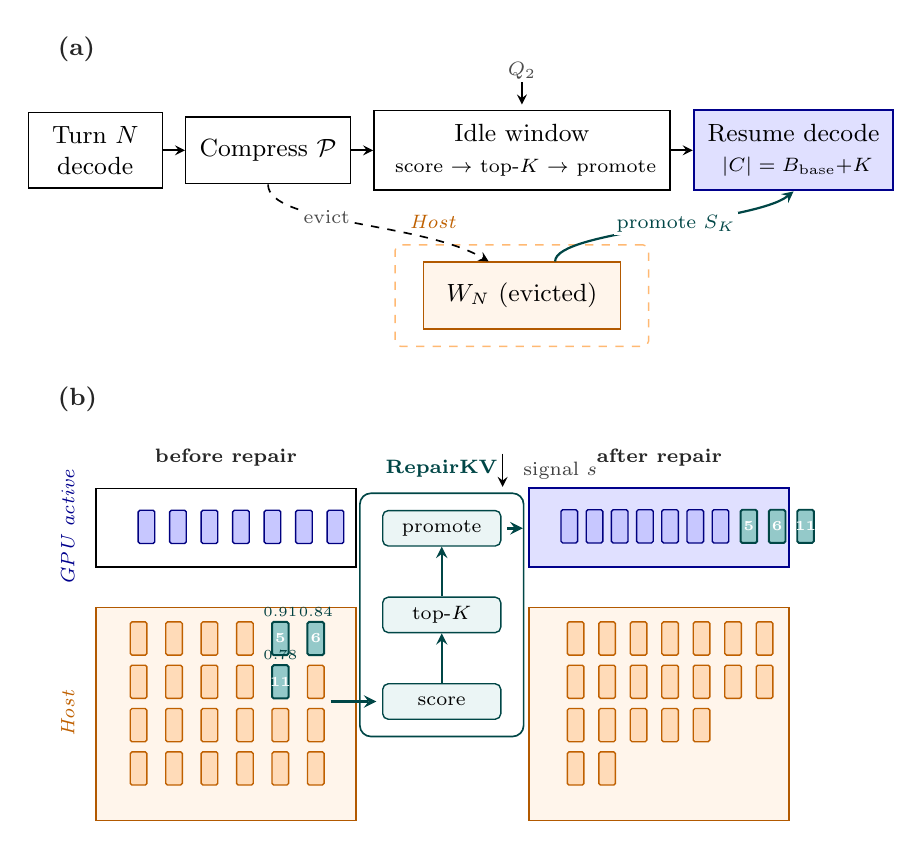
\begin{tikzpicture}[
  >=latex, line width=0.4pt,
  font=\small,
  box/.style={draw=black, fill=white, line width=0.5pt,
              inner sep=5pt, align=center, minimum height=0.85cm},
  active/.style={box, fill=blue!12, draw=blue!55!black, line width=0.7pt},
  store/.style={box, fill=orange!8, draw=orange!70!black},
  arr/.style={->, line width=0.6pt, draw=black, >=stealth},
  promarr/.style={->, line width=0.8pt, draw=teal!55!black, >=stealth},
  arrlabel/.style={font=\scriptsize, text=black!70, fill=white, inner sep=1pt},
  groupbox/.style={draw=orange!55, dashed, line width=0.5pt, rounded corners=2pt},
  grouplabel/.style={font=\scriptsize\itshape, text=orange!75!black},
  panellabel/.style={font=\bfseries\small, text=black!85},
  % Slightly wider chips so a small index numeral fits inside.
  chip/.style={rounded corners=0.6pt, minimum width=6pt, minimum height=12pt,
               inner sep=0pt, line width=0.5pt},
  gpuchip/.style={chip, draw=blue!50!black, fill=blue!22},
  hostchip/.style={chip, draw=orange!75!black, fill=orange!28},
  promchip/.style={chip, draw=teal!55!black, fill=teal!42, line width=0.7pt},
  rkvmod/.style={draw=teal!55!black, fill=teal!8, line width=0.5pt,
                 rounded corners=2pt, inner sep=3pt, align=center,
                 font=\scriptsize, minimum width=1.5cm, minimum height=0.45cm},
  rowlabel/.style={font=\itshape\scriptsize},
  bigpromarr/.style={->, line width=1.0pt, draw=teal!55!black, >=stealth},
  idxlabel/.style={font=\fontsize{4.6}{5}\selectfont, text=black!85,
                   inner sep=0pt},
  idxlabelwhite/.style={font=\fontsize{4.6}{5}\selectfont\bfseries,
                        text=white, inner sep=0pt},
  scorelabel/.style={font=\fontsize{5.4}{6}\selectfont, text=teal!50!black,
                     inner sep=0.5pt}
]
  % =================================================================
  % Panel (a) — pikv block diagram (unchanged from v1)
  % =================================================================
  \node[panellabel, anchor=south west] at (0, 4.4) {(a)};

  \node[box, minimum width=1.7cm] (dN) at (0.6, 3.4) {Turn $N$\\decode};
  \node[box, minimum width=1.6cm, right=8pt of dN] (cmp) {Compress~$\mathcal{P}$};
  \node[box, minimum width=2.5cm, right=8pt of cmp] (idle)
       {Idle window\\{\scriptsize{} score~$\to$~top-$K$~$\to$~promote}};
  \node[active, minimum width=1.9cm, right=8pt of idle] (resume)
       {Resume decode\\{\scriptsize{} $|C|=\bbase{+}K$}};

  \draw[arr] (dN) -- (cmp);
  \draw[arr] (cmp) -- (idle);
  \draw[arr] (idle) -- (resume);

  \draw[arr] ([yshift=10pt]idle.north) -- ([yshift=2pt]idle.north);
  \node[arrlabel, anchor=south] at ([yshift=10pt]idle.north) {$Q_2$};

  \node[store, minimum width=2.5cm, below=0.9cm of idle] (wn) {$W_N$ (evicted)};
  \node[groupbox, fit=(wn), inner xsep=10pt, inner ysep=6pt] (hgroup) {};
  \node[grouplabel, anchor=south west]
       at ([xshift=2pt, yshift=2pt]hgroup.north west) {Host};

  \draw[arr, dashed]
       (cmp.south) .. controls ([yshift=-0.5cm]cmp.south)
                              and ([yshift=0.5cm]wn.north west) ..
       ([xshift=-12pt]wn.north)
       node[arrlabel, pos=0.4] {evict};

  \draw[promarr]
       ([xshift=12pt]wn.north) .. controls ([xshift=12pt, yshift=0.4cm]wn.north)
                                          and ([xshift=-0.5cm, yshift=-0.4cm]resume.south) ..
       (resume.south)
       node[arrlabel, text=teal!55!black, pos=0.55] {promote~$S_K$};

  % =================================================================
  % Panel (b) — 3-column matrix with VERTICAL middle column
  % SYMMETRY: column 1 and column 3 BOTH width 3.3cm.
  % =================================================================
  \node[panellabel, anchor=south west] at (0, -0.05) {(b)};

  % Column 1 (before): x=0.6 .. 3.9   (width 3.3)
  % Column 2 (middle): x=4.2 .. 5.8   (vertical pill, width ~1.6)
  % Column 3 (after):  x=6.1 .. 9.4   (width 3.3)
  \node[box, minimum width=3.3cm, minimum height=1.0cm,
        anchor=south west] (gpuB) at (0.6, -1.9) {};
  \node[active, minimum width=3.3cm, minimum height=1.0cm,
        anchor=south west] (gpuA) at (6.1, -1.9) {};
  \node[store, minimum width=3.3cm, minimum height=2.7cm,
        anchor=north west] (hostB) at (0.6, -2.4) {};
  \node[store, minimum width=3.3cm, minimum height=2.7cm,
        anchor=north west] (hostA) at (6.1, -2.4) {};

  % Tier row labels
  \node[rowlabel, text=blue!55!black, anchor=south, rotate=90]
       at ([xshift=-4pt]gpuB.west) {GPU active};
  \node[rowlabel, text=orange!75!black, anchor=south, rotate=90]
       at ([xshift=-4pt]hostB.west) {Host};

  % Column titles
  \node[font=\bfseries\scriptsize, text=black!85, anchor=south]
       at ([yshift=4pt]gpuB.north) {before repair};
  \node[font=\bfseries\scriptsize, text=black!85, anchor=south]
       at ([yshift=4pt]gpuA.north) {after repair};

  % --- Middle column: RepairKV pill, vertical (promote at top) ---
  \node[rkvmod, anchor=center] (mpromote) at (5.0, -1.4) {promote};
  \node[rkvmod, anchor=center] (mselect)  at (5.0, -2.5) {top-$K$};
  \node[rkvmod, anchor=center] (mscore)   at (5.0, -3.6) {score};
  \draw[promarr] (mscore.north)  -- (mselect.south);
  \draw[promarr] (mselect.north) -- (mpromote.south);

  % RepairKV frame
  \node[draw=teal!55!black, line width=0.6pt, rounded corners=4pt,
        fit=(mpromote)(mscore), inner xsep=8pt, inner ysep=6pt] (rkvframe) {};
  \node[font=\scriptsize\bfseries, text=teal!55!black, anchor=south]
       at ([yshift=2pt]rkvframe.north) {\repairkv{}};

  % --- Signal s: enters TOP of the pill with short downward arrow ---
  \draw[arr] ([xshift=22pt, yshift=14pt]rkvframe.north)
             -- ([xshift=22pt, yshift=2pt]rkvframe.north);
  \node[font=\scriptsize, text=black!75, anchor=west]
       at ([xshift=26pt, yshift=8pt]rkvframe.north) {signal $s$};

  % =================================================================
  % CHIP LAYOUT — column 1 (host has 4 rows × 6 chips = 24).
  % Index numbering convention: row-major from top-left, 1..24.
  %   #5  = row 0, col 5
  %   #6  = row 0, col 6
  %   #11 = row 1, col 5
  % These are the THREE teal candidates. They reappear in GPU-after.
  % Column spacing: 0.45cm → fits inside the 3.3cm host box (chip ~6pt).
  % =================================================================

  % --- GPU before chips: 7 blue, evenly spaced inside 3.3cm box ---
  \foreach \i in {1,...,7}{
    \pgfmathsetmacro{\xc}{0.40*\i + 0.25}
    \node[gpuchip] at ([xshift=\xc cm, yshift=-0.5cm]gpuB.north west) {};
  }

  % --- GPU after chips: 7 blue (existing) + 3 numbered teal (newly promoted) ---
  \foreach \i in {1,...,7}{
    \pgfmathsetmacro{\xc}{0.32*\i + 0.20}
    \node[gpuchip] at ([xshift=\xc cm, yshift=-0.5cm]gpuA.north west) {};
  }
  % Three numbered teal chips at the right end — same identities as host.
  \pgfmathsetmacro{\xtA}{0.32*7 + 0.20 + 0.36*1}
  \pgfmathsetmacro{\xtB}{0.32*7 + 0.20 + 0.36*2}
  \pgfmathsetmacro{\xtC}{0.32*7 + 0.20 + 0.36*3}
  \node[promchip] (gpuTealA) at ([xshift=\xtA cm, yshift=-0.5cm]gpuA.north west) {};
  \node[promchip] (gpuTealB) at ([xshift=\xtB cm, yshift=-0.5cm]gpuA.north west) {};
  \node[promchip] (gpuTealC) at ([xshift=\xtC cm, yshift=-0.5cm]gpuA.north west) {};
  \node[idxlabelwhite] at (gpuTealA.center) {5};
  \node[idxlabelwhite] at (gpuTealB.center) {6};
  \node[idxlabelwhite] at (gpuTealC.center) {11};

  % =================================================================
  % --- Host before: 4 rows × 6 chips, with #5 #6 #11 as numbered teal.
  % Columns spread inside 3.3cm using 0.45cm spacing.
  % =================================================================
  \foreach \r/\rowstart in {0/1, 1/7, 2/13, 3/19}{
    \foreach \c in {1,...,6}{
      \pgfmathtruncatemacro{\idx}{\rowstart + \c - 1}
      \pgfmathsetmacro{\xh}{0.45*\c + 0.10}
      \pgfmathsetmacro{\yh}{-0.40 - 0.55*\r}
      % Skip the three teal positions — drawn separately below.
      \ifnum\idx=5\else
      \ifnum\idx=6\else
      \ifnum\idx=11\else
        \node[hostchip] at ([xshift=\xh cm, yshift=\yh cm]hostB.north west) {};
      \fi\fi\fi
    }
  }

  % Three teal candidates with identity numbers.
  % #5 → row 0 col 5;  #6 → row 0 col 6;  #11 → row 1 col 5.
  \pgfmathsetmacro{\xHa}{0.45*5 + 0.10}  \pgfmathsetmacro{\yHa}{-0.40 - 0.55*0}
  \pgfmathsetmacro{\xHb}{0.45*6 + 0.10}  \pgfmathsetmacro{\yHb}{-0.40 - 0.55*0}
  \pgfmathsetmacro{\xHc}{0.45*5 + 0.10}  \pgfmathsetmacro{\yHc}{-0.40 - 0.55*1}
  \node[promchip] (hostTealA) at ([xshift=\xHa cm, yshift=\yHa cm]hostB.north west) {};
  \node[promchip] (hostTealB) at ([xshift=\xHb cm, yshift=\yHb cm]hostB.north west) {};
  \node[promchip] (hostTealC) at ([xshift=\xHc cm, yshift=\yHc cm]hostB.north west) {};
  \node[idxlabelwhite] at (hostTealA.center) {5};
  \node[idxlabelwhite] at (hostTealB.center) {6};
  \node[idxlabelwhite] at (hostTealC.center) {11};

  % Score values above each teal candidate (small, teal-tinted).
  \node[scorelabel, anchor=south] at ([yshift=1pt]hostTealA.north) {0.91};
  \node[scorelabel, anchor=south] at ([yshift=1pt]hostTealB.north) {0.84};
  \node[scorelabel, anchor=south] at ([yshift=1pt]hostTealC.north) {0.78};

  % --- Host after: same total style as v1 but in the wider 3.3cm box.
  % 7 + 7 + 5 + 2 = 21 chips (3 fewer). The three indexed entries
  % (#5, #6, #11) are GONE from host — they live in GPU now.
  \foreach \i in {1,...,7}{
    \foreach \r in {0,1}{
      \pgfmathsetmacro{\xh}{0.40*\i + 0.20}
      \pgfmathsetmacro{\yh}{-0.40 - 0.55*\r}
      \node[hostchip] at ([xshift=\xh cm, yshift=\yh cm]hostA.north west) {};
    }
  }
  \foreach \i in {1,...,5}{
    \pgfmathsetmacro{\xh}{0.40*\i + 0.20}
    \node[hostchip] at ([xshift=\xh cm, yshift=-1.50cm]hostA.north west) {};
  }
  \foreach \i in {1,...,2}{
    \pgfmathsetmacro{\xh}{0.40*\i + 0.20}
    \node[hostchip] at ([xshift=\xh cm, yshift=-2.05cm]hostA.north west) {};
  }

  % =================================================================
  % Flow arrows (short, row-level)
  % =================================================================
  % Host candidate cluster -> SCORE (host row level).
  \draw[bigpromarr] ([xshift=2pt]hostTealB.east |- mscore)
                    -- ([xshift=-2pt]mscore.west);
  % PROMOTE -> GPU (after, left edge), GPU row level.
  \draw[bigpromarr] ([xshift=2pt]mpromote.east)
                    -- ([xshift=-2pt]gpuA.west |- mpromote);
\end{tikzpicture}
\end{document}
